\documentclass[a4paper]{scrreprt}
 
\usepackage[german]{babel}
\usepackage[utf8]{inputenc}
\usepackage[T1]{fontenc}
\usepackage{ae}
\usepackage[bookmarks,bookmarksnumbered]{hyperref}
\usepackage{graphicx}
 
\begin{document}
\title{Pflichtenheft für MensaMeat}

\maketitle
%\Footnote für Fußnoten
 
% Platzierung des Inhaltsverzeichnisses
\tableofcontents
 
\chapter{Zielbestimmung}
Mit dieser App sollen Personen(Studenten), die in der Mensa essen möchten, in die Lage versetzt werden, sich mit ihnen unbekannten Personen (Studenten) zum Essen verabreden zu können. Auf diese Art können leicht neue Menschen kennengelernt werden und keiner muss nicht alleine essen.
 
\section{Musskriterien}
\begin{itemize}


\item Erstellen und Bearbeiten eines persönlichen Profils (Nutzername(eindeutig), Alter, Geschlecht, Studiengang, Motto (Freitextfeld), Sprachen)
\item Einsehen des Mensaplans des aktuellen Tages
\item Auswählen der Mensalinien/Mensawerke
\item Einsehen der Gruppen, mit übereinstimmenden Mensalnien/Werken
\item Erstellen einer Gruppe
\item Beitreten einer Gruppe
\item Verlassen einer Gruppe
\item Anschauen der Profile der Gruppenmitglieder
\item Automatisches Löschen der Gruppe am Ende des Tages, bzw wenn letzes Mitglied austritt
\end{itemize}

\section{Wunschkriterien}
\begin{itemize}

\item Erweiterte Profileinstellungen (Mag, Mag nicht, Vegetarier/Veganer,... )
\item E-Mail Verifizierung für die Erstellung eines Profils 
\item Bitmoji erstellen, welches als Profilbild angezeigt wird
\item (gern) Ranking System um die Zuverlässigkeit einer Person einzuschätzen. Das Erscheinen zu den Treffen bringt Punkte, von denen der Rang abhängt
\item Gruppenmitglieder können angeben, welche Personen zur Verabredung erschienen bzw. nicht erschienen sind, dies wirkt sich auf das Ranking aus
\item Einstellbare Restriktionen für den Gruppenbeitritt, z.b. nach Geschlecht, Studiengang, Veganismus, Rang, Alter
\item Filtermöglichkeiten der angezeigten Gruppen z.b. nach Treffzeitpunkt, aktuelle und maximale Mitgliederanzahl 
\item Einsicht in den Mensaplan der folgenden Tage und
\item Erstellen einer Gruppe für folgende Tage
\item Melden von Personen ("Snapshot" der Sicht aus der gemeldet wird, zum beurteilen an Administratoren gesandt) 
\end{itemize}
 
\section{Abgrenzungskriterien}
\begin{itemize}

\item Kein Upload von (Profil-)Bildern möglich
\item Kein "Kicken" von Personen aus erstellter Gruppe
\item Kein Chatsystem
\item Kein Löschen von Gruppen (denn Gruppengründer hat gleichwertige Rolle zu anderen Mitgliedern, er kann selbst austreten.)

\end{itemize}
 
\chapter{Produkteinsatz}
Das Produkt wird von Personen(Studenten) eingesetzt, um sich mit unbekannte Personen (Studenten) zum gemeinsamen Essen in der Mensa zu verabreden.

 
\section{Anwendungsbereiche}
Essensplanung an der Mensa (Wann, mit Wem, an welche Linie).
 
\section{Zielgruppen}
Mensagänger; Studenten, Professoren, Auszubildende 
 
\section{Betriebsbedingungen}
\subsection{Physikalische Umgebung}
Zuhause, Campus, Unterwegs(in der Stadt, in der Straßenbahn)

\subsection{Tägliche Betriebszeit}
erwartet bis zu 3 mal täglich, jeweils weniger als 10 Minuten am Stück 
 
\chapter{Produktumgebung}
Das Produkt läuft als App auf einem Smartphone

\section{Software}
Android, ab Version 4.4?
 
\section{Hardware}
Smartphone 
 
\section{Orgware}

\section{Produktschnittstellen} 
 
\chapter{Funktionale Anforderungen}
TODO Sie werden eingeteilt in Client und Server Funktionalitäten.

\section{Client}
Auf dem Client (in diesem Fall ein Smartphone) müssen alle folgende Anforderungen erfüllt sein. 

\subsection{Allgemein}

\begin{addmargin}[25pt]{0pt} 
\textbf{/CAFA10/} Installation der Applikation \\
\textbf{/CAFA20/} Starten / Beenden der Applikation\\
\textbf{/CAFA30/} Speciherung lokaler Daten (Login Daten)\\
\end{addmargin}

\subsection{User Interface}

\begin{addmargin}[25pt]{0pt} 
\textbf{/CIFA10/} Anmelden / Registrieren \\
Es muss eine Seite geben auf der Buttons für Anmeldung und Registrierung sind.
\textbf{/CIFA20/} Angaben persönlicher Daten\\
\textbf{/CIFA30/} Anzeigen und Auswählen der Essenslinien\\
\textbf{/CIFA40/} Angeben des bevorzugten Zeitraums\\
\textbf{/CIFA50/} Anzeigen und Auswählen einer Gruppe\\
\textbf{/CIFA60/} Anzeigen eines Userprofils\\
Anzeigen des Regelwerks\\
Anzeigen der Gruppenseite\\
Einstellngen des Profils\\
\end{addmargin}

\section{Server}

\begin{addmargin}[25pt]{0pt} 
\textbf{/SFA10/} User anlegen / löschen\\
\textbf{/SFA20/} User anmelden / abmelden\\
\textbf{/SFA30/} Gruppe erstellen mit Parametern\\
\textbf{/SFA40/} Gruppe löschen\\
	\begin{addmargin}[25pt]{0pt} 
	\textbf{/SFA41/} Durch Autretten des letzten Users\\
	\textbf{/SFA41/} Durch Admin\\
	\textbf{/SFA42/} Automatisch durch Timeout\\
	\end{addmargin}
\textbf{/SFA41/} Anzeigen der Gruppen zu Parametern\\
\textbf{/SFA120/} User tritt Gruppe bei\\
\textbf{/SFA130/} User verlässt Gruppe\\
\textbf{/SFA130/} Informationen bearbeiten von User\\
\textbf{/SFA120/} Abfragen der Mensapläne\\
\textbf{/SFA41/} Abfragen von Userprofil\\
\end{addmargin}

\chapter{Produktdaten}

\section{Benutzerdaten}

\begin{addmargin}[25pt]{0pt}
\textbf{/D10/} Über einen Benutzer der App sind folgende Daten zu speichern:\\
Benutzername, Passwort, (E-Mail), ALTER?, Profilbild, Motto, Geschlecht, STATUS?(Student, Prof., Sonstiges), Essenspräferenzen, Administratorfunktionen\\
\textbf{/D20/} Handelt es sich um einen Benutzer des Status Student, so ist zusätzlich der Studiengang zu erfassen\\
\textbf{/D30/} Während der Nutzung der Applikation werden Statistiken anhand folgender Daten erhoben:\\
Anzahl der erstellten Gruppen, Anzahl der Gruppenbeitritte, Anzahl der Gruppenaustritte, Anzahl der erfolgreichen Treffen\\
\end{addmargin}

\section{Gruppendaten}

\begin{addmargin}[25pt]{0pt}
\textbf{/D40/} Über jede erstellte Gruppe sind folgende Daten zu speichern:\\
Gruppenname, Motto, Essenslinie, Uhrzeit, Teilnehmeranzahl, Gruppenmitglieder\\
\end{addmargin}

\section{Mensadaten}

\begin{addmargin}[25pt]{0pt}
\textbf{/D50} Die zu speichernden Mensadaten beinhalten lediglich den tagesaktuellen Speiseplan\\
\end{addmargin}



\chapter{Nichtfunktionale Anforderungen}

\begin{addmargin}[25pt]{0pt} 

\textbf{/NFA10/} Es können bis zu 10.000 User in der Datenbank angelegt werden.\\
\textbf{/NFA20/} Eingaben dürfen nicht länger als 255 Zeiche sein.\\
\textbf{/NFA30/} Benutzernamen dürfen nicht länger als 40 Zeiche sein.\\
\textbf{/NFA40/} Es können beim Suchen passender Gruppen bis zu 24 Ergebnisse geliefert werden, um die Serverauslastung zu minimieren.\\
\textbf{/NFA50/} Serverarbeiten fidnen nur zwischen 0:00 und 6:00 Uhr statt.\\
\textbf{/NFA70/} Das System muss parallel von bis zu 1000 Usern benutzt werden können.\\
\textbf{/NFA80/} Das System darf nicht mehr als einen Neustart pro Woche brauchen.\\
\textbf{/NFA90/} Es soll ab Öffnen der App in 6 Klicks möglich sein einer Gruppe beizutreten.\\
\textbf{/NFA100/} Alle Buttons sollen gut lesbar und leicht anklickbar sein.\\

\end{addmargin}


\chapter{Globale Testfälle}
\begin{addmargin}[25pt]{0pt} 
\textbf{/T10/} Ein nicht registrierter Nutzer öffnet die App, registriert sich erfolgreich und gelangt auf die „Profil Bearbeiten“-Seite\\
  \begin{addmargin}[25pt]{0pt} 
  \textbf{/T110/} Bearbeitet dieser sein Profil vollständig, ist der Registrierungsprozess abgeschlossen und ihm stehen alle Funktionen zur Verfügung\\
  \textbf{/T120/} Schließt dieser die Applikation, so wird er beim erneuten Öffnen direkt zur Profilbearbeitung weitergeleitet. Wiederholen bis erfolgreich abgeschlossen.\\
  \end{addmargin}
\textbf{/T20/}  Ein registrierter Nutzer öffnet die App und betrachtet die Essenmöglichkeiten des aktuellen Tages\\
\textbf{/T30/} Auswahl einer Linie und Uhrzeit sowie der Beitritt einer vorgeschlagenen Gruppe\\
  \begin{addmargin}[25pt]{0pt} 
  \textbf{/T310/} Erfolgreiche Teilnahme am Gruppentreffen\\
  \textbf{/T320/} Vorzeitiger Austritt aus der Gruppe und das anschließenden Anzeigen der Homeseite\\
  \end{addmargin}
\textbf{/T40/}  Erstellungsprozess einer Gruppe\\
  \begin{addmargin}[25pt]{0pt} 
  \textbf{/T410/} Erfolgreiche Erstellung durch Eingabe aller erforderlichen Daten\\
  \textbf{/T420/} Absichtlicher Abbruch des Erstellungsprozess\\
  \textbf{/T430/} Erstellung wird durch fehlende Parameter nicht beendet\\
  \end{addmargin}
\textbf{/T50/} Ein Administrator öffnet die App und gelangt auf die Adminseite\\
  \begin{addmargin}[25pt]{0pt} 
  \textbf{/T510/} Administrator löscht Gruppe\\
  \textbf{/T520/} Administrator löscht Benutzer\\
  \end{addmargin}



\end{addmargin}

\chapter{Systemmodelle}
\section{Anwendungsfalldiagramm}	

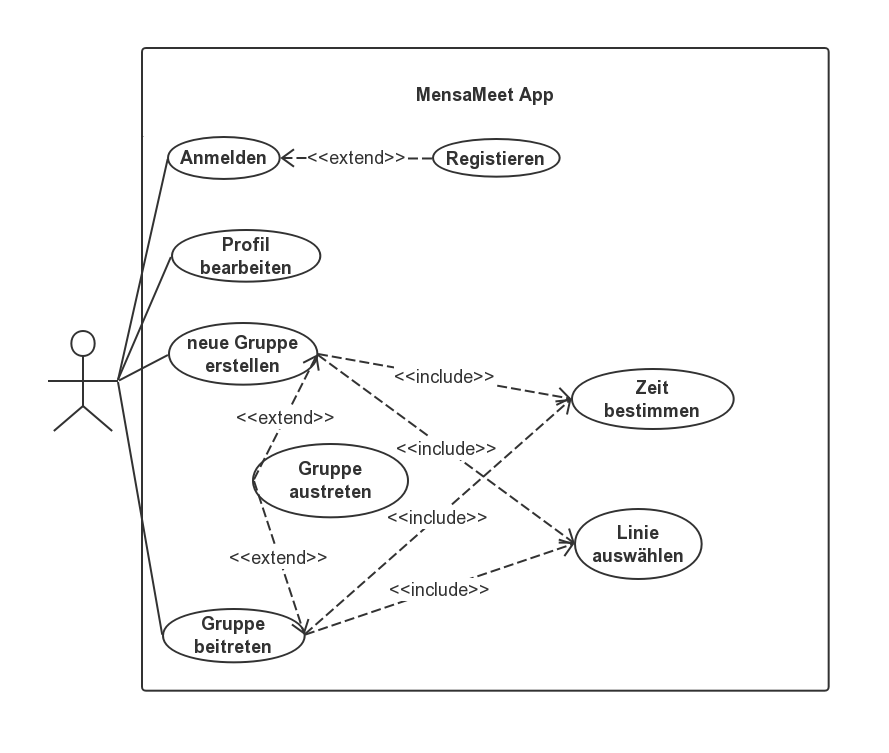
\includegraphics[scale=0.6]{userCase.jpg}


\chapter{Glossar}
 

 


\end{document}